\documentclass[aspectratio=169,10pt]{beamer}

\usepackage[T1]{fontenc}
\usepackage[utf8]{inputenc}
\usepackage{booktabs}
\usepackage{xcolor}
\usepackage{colortbl}
\usepackage{graphicx}
\usepackage{tikz}
\usetikzlibrary{arrows.meta,positioning}

% Speaker notes are hidden by default. Swap to `show notes` for a presenter build
% (produces one notes page after each slide).
\setbeameroption{hide notes}

\usetheme{default}
\usefonttheme{professionalfonts}
\usepackage{helvet}
\renewcommand{\familydefault}{\sfdefault}
\setbeamertemplate{navigation symbols}{}

% ---------------------------------------------------------------- palette
% Lifted from frontend/src/styles.css so the deck matches the product UI.
\definecolor{arBg}{HTML}{050914}
\definecolor{arPanel}{HTML}{0D1623}
\definecolor{arPanel2}{HTML}{111B2B}
\definecolor{arBorder}{HTML}{2A3849}
\definecolor{arText}{HTML}{EDF3F8}
\definecolor{arMuted}{HTML}{9AAEC5}
\definecolor{arFaint}{HTML}{62748C}
\definecolor{arCyan}{HTML}{5B8DEF}
\definecolor{arCyan2}{HTML}{9FC0FF}
\definecolor{arGreen}{HTML}{4FD1A1}
\definecolor{arAmber}{HTML}{E1AD58}
\definecolor{arDanger}{HTML}{F97066}

\setbeamercolor{background canvas}{bg=arBg}
\setbeamercolor{normal text}{fg=arText}
\setbeamercolor{structure}{fg=arCyan}
\setbeamercolor{itemize item}{fg=arCyan}
\setbeamercolor{itemize subitem}{fg=arMuted}
\setbeamercolor{enumerate item}{fg=arCyan}
\setbeamertemplate{itemize items}[circle]

\setbeamercolor{panel}{bg=arPanel,fg=arText}
\setbeamercolor{panelglow}{bg=arPanel2,fg=arText}

\setbeamerfont{frametitle}{size=\LARGE,series=\bfseries}
\setbeamercolor{frametitle}{fg=arText}

\arrayrulecolor{arBorder}

% ---------------------------------------------------------------- helpers
\newcommand{\eyebrow}[1]{%
  {\color{arCyan2}\fontsize{6.6}{8}\selectfont\bfseries\MakeUppercase{#1}}}
\newcommand{\cy}[1]{{\color{arCyan2}\bfseries #1}}
\newcommand{\gn}[1]{{\color{arGreen}\bfseries #1}}
\newcommand{\am}[1]{{\color{arAmber}\bfseries #1}}
\newcommand{\muted}[1]{{\color{arMuted} #1}}
\newcommand{\faint}[1]{{\color{arFaint}\small #1}}
\newcommand{\plabel}[1]{{\color{arCyan2}\fontsize{6.4}{7.6}\selectfont\bfseries\MakeUppercase{#1}}}
\newcommand{\plabelam}[1]{{\color{arAmber}\fontsize{6.4}{7.6}\selectfont\bfseries\MakeUppercase{#1}}}
\newcommand{\plabelgn}[1]{{\color{arGreen}\fontsize{6.4}{7.6}\selectfont\bfseries\MakeUppercase{#1}}}
\newcommand{\ptitle}[1]{{\color{arText}\large\bfseries #1}}

% rounded panel: \panel{width}{content}
\newenvironment{panel}[1]{%
  \begin{beamercolorbox}[wd=#1,rounded=true,shadow=false,sep=7pt]{panel}%
}{%
  \end{beamercolorbox}%
}
\newenvironment{panelglow}[1]{%
  \begin{beamercolorbox}[wd=#1,rounded=true,shadow=false,sep=7pt]{panelglow}%
}{%
  \end{beamercolorbox}%
}

% stat tile
\newcommand{\stat}[2]{%
  \begin{minipage}[t]{0.30\linewidth}
    \begin{beamercolorbox}[wd=\linewidth,rounded=true,shadow=false,sep=7pt]{panel}
      {\color{arCyan}\fontsize{24}{26}\selectfont\bfseries #1}\\[0.3em]
      {\color{arMuted}\footnotesize #2}
    \end{beamercolorbox}
  \end{minipage}%
}

\makeatletter
\setbeamertemplate{frametitle}{%
  \vspace{0.25em}%
  \begin{beamercolorbox}[wd=\textwidth]{frametitle}
    \eyebrow{\insertframesubtitle}\\[0.35em]
    \usebeamerfont{frametitle}\usebeamercolor[fg]{frametitle}\insertframetitle
  \end{beamercolorbox}%
  \vspace{-0.3em}
}
\makeatother

\setbeamertemplate{footline}{%
  \hbox{\begin{beamercolorbox}[wd=\paperwidth,ht=2.6ex,dp=1.6ex,leftskip=1.5em,rightskip=1.5em]{}%
    {\color{arFaint}\scriptsize\bfseries AdaptiveRoute \textperiodcentered\ Proof of Concept}%
    \hfill{\color{arMuted}\scriptsize\bfseries\insertframenumber\,/\,17}%
  \end{beamercolorbox}}%
}

\begin{document}

% ================================================================ 1 title
{
\setbeamertemplate{footline}{}
\begin{frame}[plain]
  \vspace{0.6em}
  
\begin{tikzpicture}[baseline]
    \node[draw=arCyan!55,rounded corners=7pt,fill=arPanel2,minimum width=11mm,minimum height=11mm] (m) at (0,0) {};
    \begin{scope}[shift={(m.center)},scale=0.030,yscale=-1,draw=arCyan,line width=2.2pt,
                  line cap=round,line join=round]
      \draw (-6,7) circle (3);
      \draw (-3,7) -- (5.5,7);
      \draw[rounded corners=2] (5.5,7) .. controls (9,7) and (9,0) .. (5.5,0) -- (-5.5,0)
            .. controls (-9,0) and (-9,-7) .. (-5.5,-7) -- (3,-7);
      \draw (6,-7) circle (3);
    \end{scope}
  \end{tikzpicture}\hspace{0.5em}
  \begin{minipage}[b]{0.5\linewidth}
    {\color{arText}\bfseries AdaptiveRoute}\\[0.15em]
    {\color{arMuted}\small Operational route intelligence}
  \end{minipage}

  \vspace{1.9em}
  {\fontsize{40}{42}\selectfont\bfseries\color{arText} Agentic\\[0.08em] replanning}

  \vspace{0.8em}
  {\fontsize{15}{19}\selectfont\color{arMuted}
   A fine-tuned routing policy for speed.\\ A MILP solver for the guarantee.}

  \vspace{1.7em}
  \begin{beamercolorbox}[wd=4.6cm,rounded=true,shadow=false,sep=4pt,center]{panelglow}
    {\color{arCyan2}\scriptsize\bfseries PROOF OF CONCEPT \textperiodcentered\ 5 DAYS}
  \end{beamercolorbox}
  \vspace{0.5em}
  {\color{arMuted}\small Gabriel Carvalho Domingos da Conceição}
\end{frame}
}

% ================================================================ 2 problem
\begin{frame}
  \frametitle{Routes are planned once.\\ Reality changes all day.}
  \framesubtitle{AdaptiveRoute \textperiodcentered\ The problem}

  \vspace{0.2em}
  \muted{A delivery route is optimised the night before. By mid-morning it is already wrong.}

  \vspace{1.0em}
  \begin{columns}[T]
    \begin{column}{0.315\linewidth}
      \begin{panel}{\linewidth}
        \plabel{Network}\\[0.5em]
        \ptitle{A road closes}\\[0.45em]
        \muted{\small An accident blocks the segment the driver was routed through.}
      \end{panel}
    \end{column}
    \begin{column}{0.315\linewidth}
      \begin{panel}{\linewidth}
        \plabel{Demand}\\[0.5em]
        \ptitle{A customer cannot receive}\\[0.45em]
        \muted{\small Store shut, nobody on site, delivery window missed.}
      \end{panel}
    \end{column}
    \begin{column}{0.315\linewidth}
      \begin{panel}{\linewidth}
        \plabel{Priority}\\[0.5em]
        \ptitle{The order changes}\\[0.45em]
        \muted{\small A delivery becomes urgent after the plan was frozen.}
      \end{panel}
    \end{column}
  \end{columns}

  \vspace{0.9em}
  \centering
  \small Today the driver phones an operator, who re-plans by hand.
  \textbf{The optimisation asset built overnight is abandoned by 10am.}
\end{frame}

% ================================================================ 3 tension
\begin{frame}
  \frametitle{Two obvious approaches,\\ each with a disqualifying flaw}
  \framesubtitle{AdaptiveRoute \textperiodcentered\ Why this is hard}

  \vspace{0.7em}
  \begin{columns}[T]
    \begin{column}{0.478\linewidth}
      \begin{panel}{\linewidth}
        \plabel{Option A}\\[0.5em]
        \ptitle{Ask a language model}\\[0.5em]
        \muted{\small Speaks the driver's language. Answers in seconds.}\\[0.6em]
        {\small \am{But:} no notion of capacity. It will route straight through the blocked road.}
      \end{panel}
    \end{column}
    \begin{column}{0.478\linewidth}
      \begin{panel}{\linewidth}
        \plabel{Option B}\\[0.5em]
        \ptitle{Re-run the optimiser}\\[0.5em]
        \muted{\small Provably correct. Respects every constraint.}\\[0.6em]
        {\small \am{But:} it needs a formal model of the disruption, not a sentence.}
      \end{panel}
    \end{column}
  \end{columns}

  \vspace{0.8em}
  \centering
  \small The gap is not optimisation, and not language. \cy{It is the handoff.}

  \note{Plausible output is not feasible output --- the model produces something that reads like a
  route but violates capacity or skips a customer. The optimiser has the opposite problem: correct
  answers to a question nobody asked it, because someone still has to translate ``there was an
  accident between C7 and C6'' into a blocked arc before it can run.}
\end{frame}

% ================================================================ 4 thesis
{
\setbeamertemplate{frametitle}{}
\begin{frame}
  \vspace{1.2em}
  \centering
  \eyebrow{AdaptiveRoute \textperiodcentered\ Design thesis}

  \vspace{1.5em}
  {\fontsize{27}{33}\selectfont\bfseries\color{arText} The model proposes.}\\[0.25em]
  {\fontsize{27}{33}\selectfont\bfseries\color{arCyan2} The solver decides.}

  \vspace{1.8em}
  \begin{panelglow}{0.80\linewidth}
    \raggedright\small
    The fine-tuned model is treated as a \cy{fast candidate generator}, never as an authority.
    Every plan it produces is parsed, checked against deterministic rules, repaired if it can be
    repaired safely, and replaced by the MILP solver if it cannot.

    \vspace{0.7em}
    Nothing reaches the driver without passing the same validation gate ---
    \textbf{regardless of who produced it}.
  \end{panelglow}
\end{frame}
}

% ================================================================ 5 two models
\begin{frame}
  \frametitle{Breadth where the problem is open.\\ Precision where it is narrow.}
  \framesubtitle{AdaptiveRoute \textperiodcentered\ Two models, two jobs}

  \vspace{0.7em}
  \begin{columns}[T]
    \begin{column}{0.478\linewidth}
      \begin{panel}{\linewidth}
        {\color{arFaint}\scriptsize\bfseries ORCHESTRATOR \textperiodcentered\ OFF THE SHELF}\\[0.5em]
        {\color{arText}\Large\bfseries Qwen2.5-Coder-32B}\\[0.6em]
        \muted{\small Reads the driver's message, extracts the operational event, answers questions
        about the route.}\\[0.7em]
        \faint{general purpose \textperiodcentered\ temperature 0.1}
      \end{panel}
    \end{column}
    \begin{column}{0.478\linewidth}
      \begin{panelglow}{\linewidth}
        {\color{arCyan2}\scriptsize\bfseries ROUTING POLICY \textperiodcentered\ FINE-TUNED}\\[0.5em]
        {\color{arText}\Large\bfseries Qwen2.5-7B \color{arCyan2}+ LoRA v5}\\[0.6em]
        \muted{\small Emits the sequence of stops. Nothing else. Trained on the solver's own output.}\\[0.7em]
        \faint{specialised \textperiodcentered\ temperature 0}
      \end{panelglow}
    \end{column}
  \end{columns}

  \vspace{1.1em}
  \centering
  The 32B never touches a route. \cy{The 7B never talks to a driver.}

  \note{This is a right-sizing argument. Language understanding is open-ended and needs breadth, so
  it gets a large general model off the shelf. Emitting a valid route JSON is a narrow structured
  task that needs precision and speed, so it gets a small fine-tuned specialist --- and it sits on
  the hot path, so you are not paying 32B inference for every candidate. The two are configured
  independently: separate base URLs, models and temperatures.}
\end{frame}

% ================================================================ 6 architecture
\begin{frame}
  \frametitle{FastAPI core, pluggable\\ everywhere it matters}
  \framesubtitle{AdaptiveRoute \textperiodcentered\ Architecture}

  \vspace{0.1em}
  \centering
  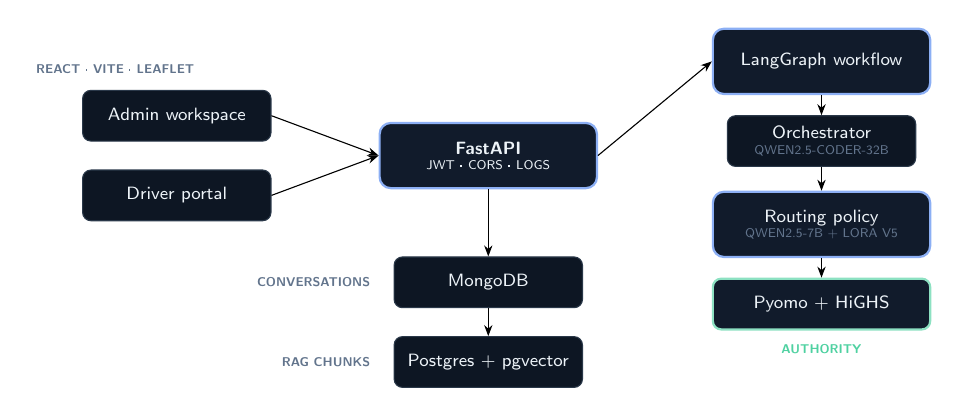
\begin{tikzpicture}[
    scale=0.92,transform shape,
    font=\scriptsize,
    box/.style={draw=arBorder,fill=arPanel,rounded corners=3pt,minimum height=7mm,
                minimum width=26mm,align=center,text=arText},
    core/.style={draw=arCyan!70,line width=0.8pt,fill=arPanel2,rounded corners=4pt,
                 minimum height=9mm,minimum width=30mm,align=center,text=arText},
    auth/.style={draw=arGreen!65,line width=0.8pt,fill=arPanel2,rounded corners=3pt,
                 minimum height=7mm,minimum width=30mm,align=center,text=arText},
    lbl/.style={text=arFaint,font=\tiny\bfseries},
    ok/.style={text=arGreen,font=\tiny\bfseries},
    ar/.style={-{Stealth[length=4pt]},draw=arBorder!180}
  ]
    \node[lbl] at (-3.05,3.15) {REACT \textperiodcentered\ VITE \textperiodcentered\ LEAFLET};
    \node[box] (admin)  at (-2.2,2.5) {Admin workspace};
    \node[box] (driver) at (-2.2,1.4) {Driver portal};

    \node[core] (api) at (2.1,1.95) {\textbf{FastAPI}\\[-2pt]\tiny JWT \textperiodcentered\ CORS \textperiodcentered\ LOGS};

    \node[core] (graph)  at (6.7,3.25) {LangGraph workflow};
    \node[box]  (orch)   at (6.7,2.15) {Orchestrator\\[-2pt]\tiny\color{arFaint}QWEN2.5-CODER-32B};
    \node[core] (policy) at (6.7,1.0)  {Routing policy\\[-2pt]\tiny\color{arFaint}QWEN2.5-7B + LORA V5};
    \node[auth] (solver) at (6.7,-0.1) {Pyomo + HiGHS};
    \node[ok] at (6.7,-0.72) {AUTHORITY};

    \node[box] (mongo) at (2.1,0.2)  {MongoDB};
    \node[box] (pg)    at (2.1,-0.9) {Postgres + pgvector};
    \node[lbl,left=2mm of mongo] {CONVERSATIONS};
    \node[lbl,left=2mm of pg]    {RAG CHUNKS};

    \draw[ar] (admin.east)  -- (api.west);
    \draw[ar] (driver.east) -- (api.west);
    \draw[ar] (api.east)    -- (graph.west);
    \draw[ar] (graph.south) -- (orch.north);
    \draw[ar] (orch.south)  -- (policy.north);
    \draw[ar] (policy.south)-- (solver.north);
    \draw[ar] (api.south)   -- (mongo.north);
    \draw[ar] (mongo.south) -- (pg.north);
  \end{tikzpicture}

  \vspace{0.5em}
  \faint{Engine, policy and event extractor are swappable by environment variable.
  Tests run in-memory --- no GPU, no database, no model server.}
\end{frame}

% ================================================================ 6 cascade
\begin{frame}
  \frametitle{Each stage is slower and more\\ trustworthy than the one above it}
  \framesubtitle{AdaptiveRoute \textperiodcentered\ The replanning cascade}

  \centering
  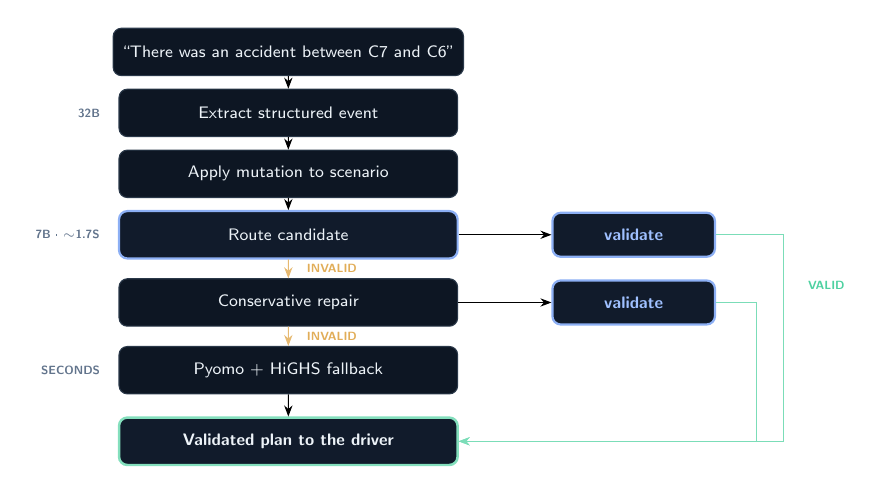
\begin{tikzpicture}[
    scale=0.86,transform shape,
    font=\scriptsize,
    box/.style={draw=arBorder,fill=arPanel,rounded corners=3pt,minimum height=7mm,
                minimum width=50mm,align=center,text=arText},
    core/.style={draw=arCyan!70,line width=0.8pt,fill=arPanel2,rounded corners=3pt,
                 minimum height=7mm,minimum width=50mm,align=center,text=arText},
    gate/.style={draw=arCyan!70,line width=0.8pt,fill=arPanel2,rounded corners=3pt,
                 minimum height=6.5mm,minimum width=24mm,align=center,text=arCyan2,font=\scriptsize\bfseries},
    auth/.style={draw=arGreen!70,line width=0.9pt,fill=arPanel2,rounded corners=3pt,
                 minimum height=7mm,minimum width=50mm,align=center,text=arText,font=\scriptsize\bfseries},
    lbl/.style={text=arFaint,font=\tiny\bfseries},
    ok/.style={draw=arGreen!75,-{Stealth[length=4pt]},text=arGreen,font=\tiny\bfseries},
    oklbl/.style={text=arGreen,font=\tiny\bfseries},
    no/.style={draw=arAmber!85,-{Stealth[length=4pt]},text=arAmber,font=\tiny\bfseries},
    ar/.style={-{Stealth[length=4pt]},draw=arBorder!180}
  ]
    \node[box]  (msg)   at (0,4.0)  {``There was an accident between C7 and C6''};
    \node[box]  (extr)  at (0,3.1)  {Extract structured event};
    \node[box]  (mut)   at (0,2.2)  {Apply mutation to scenario};
    \node[core] (cand)  at (0,1.3)  {Route candidate};
    \node[lbl,left=1.5mm of extr] {32B};
    \node[box]  (rep)   at (0,0.3)  {Conservative repair};
    \node[box]  (fall)  at (0,-0.7) {Pyomo + HiGHS fallback};
    \node[auth] (final) at (0,-1.75){Validated plan to the driver};

    \node[gate] (g1) at (5.1,1.3) {validate};
    \node[gate] (g2) at (5.1,0.3) {validate};

    \node[lbl,left=1.5mm of cand] {7B \textperiodcentered\ $\sim$1.7S};
    \node[lbl,left=1.5mm of fall] {SECONDS};

    \draw[ar] (msg)  -- (extr);
    \draw[ar] (extr) -- (mut);
    \draw[ar] (mut)  -- (cand);
    \draw[no] (cand) -- (rep)  node[midway,right=1.5mm] {INVALID};
    \draw[no] (rep)  -- (fall) node[midway,right=1.5mm] {INVALID};
    \draw[ar] (fall) -- (final);

    \draw[ar] (cand.east) -- (g1.west);
    \draw[ar] (rep.east)  -- (g2.west);

    \draw[ok] (g1.east) -- ++(1.0,0) |- (final.east);
    \draw[ok] (g2.east) -- ++(0.6,0) |- (final.east);
    \node[oklbl,anchor=west] at (7.55,0.55) {VALID};
  \end{tikzpicture}

  \vspace{0.2em}
  \faint{When the existing plan survives the event, it is reused and the model is never called.}
\end{frame}

% ================================================================ 7 validation
\begin{frame}
  \frametitle{One arbiter, independent\\ of who wrote the plan}
  \framesubtitle{AdaptiveRoute \textperiodcentered\ The validation contract}

  \vspace{0.5em}
  \begin{panel}{\linewidth}
    \plabel{A plan is accepted only if every rule holds}\\[0.7em]
    \begin{minipage}[t]{0.47\linewidth}
      \begin{itemize}\setlength\itemsep{0.3em}
        \item[\color{arCyan}$\bullet$] Every active customer visited \cy{exactly once}
        \item[\color{arCyan}$\bullet$] Each route starts and ends at the depot
        \item[\color{arCyan}$\bullet$] Vehicle capacity respected
      \end{itemize}
    \end{minipage}\hfill
    \begin{minipage}[t]{0.47\linewidth}
      \begin{itemize}\setlength\itemsep{0.3em}
        \item[\color{arCyan}$\bullet$] No blocked arc traversed
        \item[\color{arCyan}$\bullet$] Only known vehicles and active customers
        \item[\color{arCyan}$\bullet$] No duplicate or inactive stops
      \end{itemize}
    \end{minipage}
  \end{panel}

  \vspace{0.6em}
  \begin{columns}[T]
    \begin{column}{0.47\linewidth}
      \plabelgn{Numbers cannot be hallucinated}\\[0.5em]
      \muted{\small The validator \gn{recomputes} load and distance.}
    \end{column}
    \begin{column}{0.47\linewidth}
      \plabelgn{Failure is a prompt, not an error}\\[0.5em]
      \muted{\small Violations feed back. Three attempts, then the solver.}
    \end{column}
  \end{columns}

  \note{The model supplies only the visit sequence --- every number in the final plan is recomputed
  from the scenario, so a hallucinated distance cannot survive. When validation fails, the specific
  violations (``capacity\_violation: load 45, capacity 40'') are fed back as a structured correction
  prompt rather than a generic retry.}
\end{frame}

% ================================================================ 9 product
% Accent bar + text. The rule is drawn with a negative depth so it spans the
% whole block instead of sitting on the last baseline.
\newcommand{\callout}[2]{%
  \noindent
  {\color{arCyan}\rule[-4.2ex]{1.2pt}{6.0ex}}\hspace{0.6em}%
  \begin{minipage}[t]{0.86\linewidth}
    \raggedright
    {\color{arText}\small\bfseries #1}\\[0.3em]
    \muted{\scriptsize #2}
  \end{minipage}}

\begin{frame}
  \frametitle{Admin console}
  \framesubtitle{AdaptiveRoute \textperiodcentered\ The product}

  \vspace{0.3em}
  \begin{columns}[c]
    \begin{column}{0.72\linewidth}
      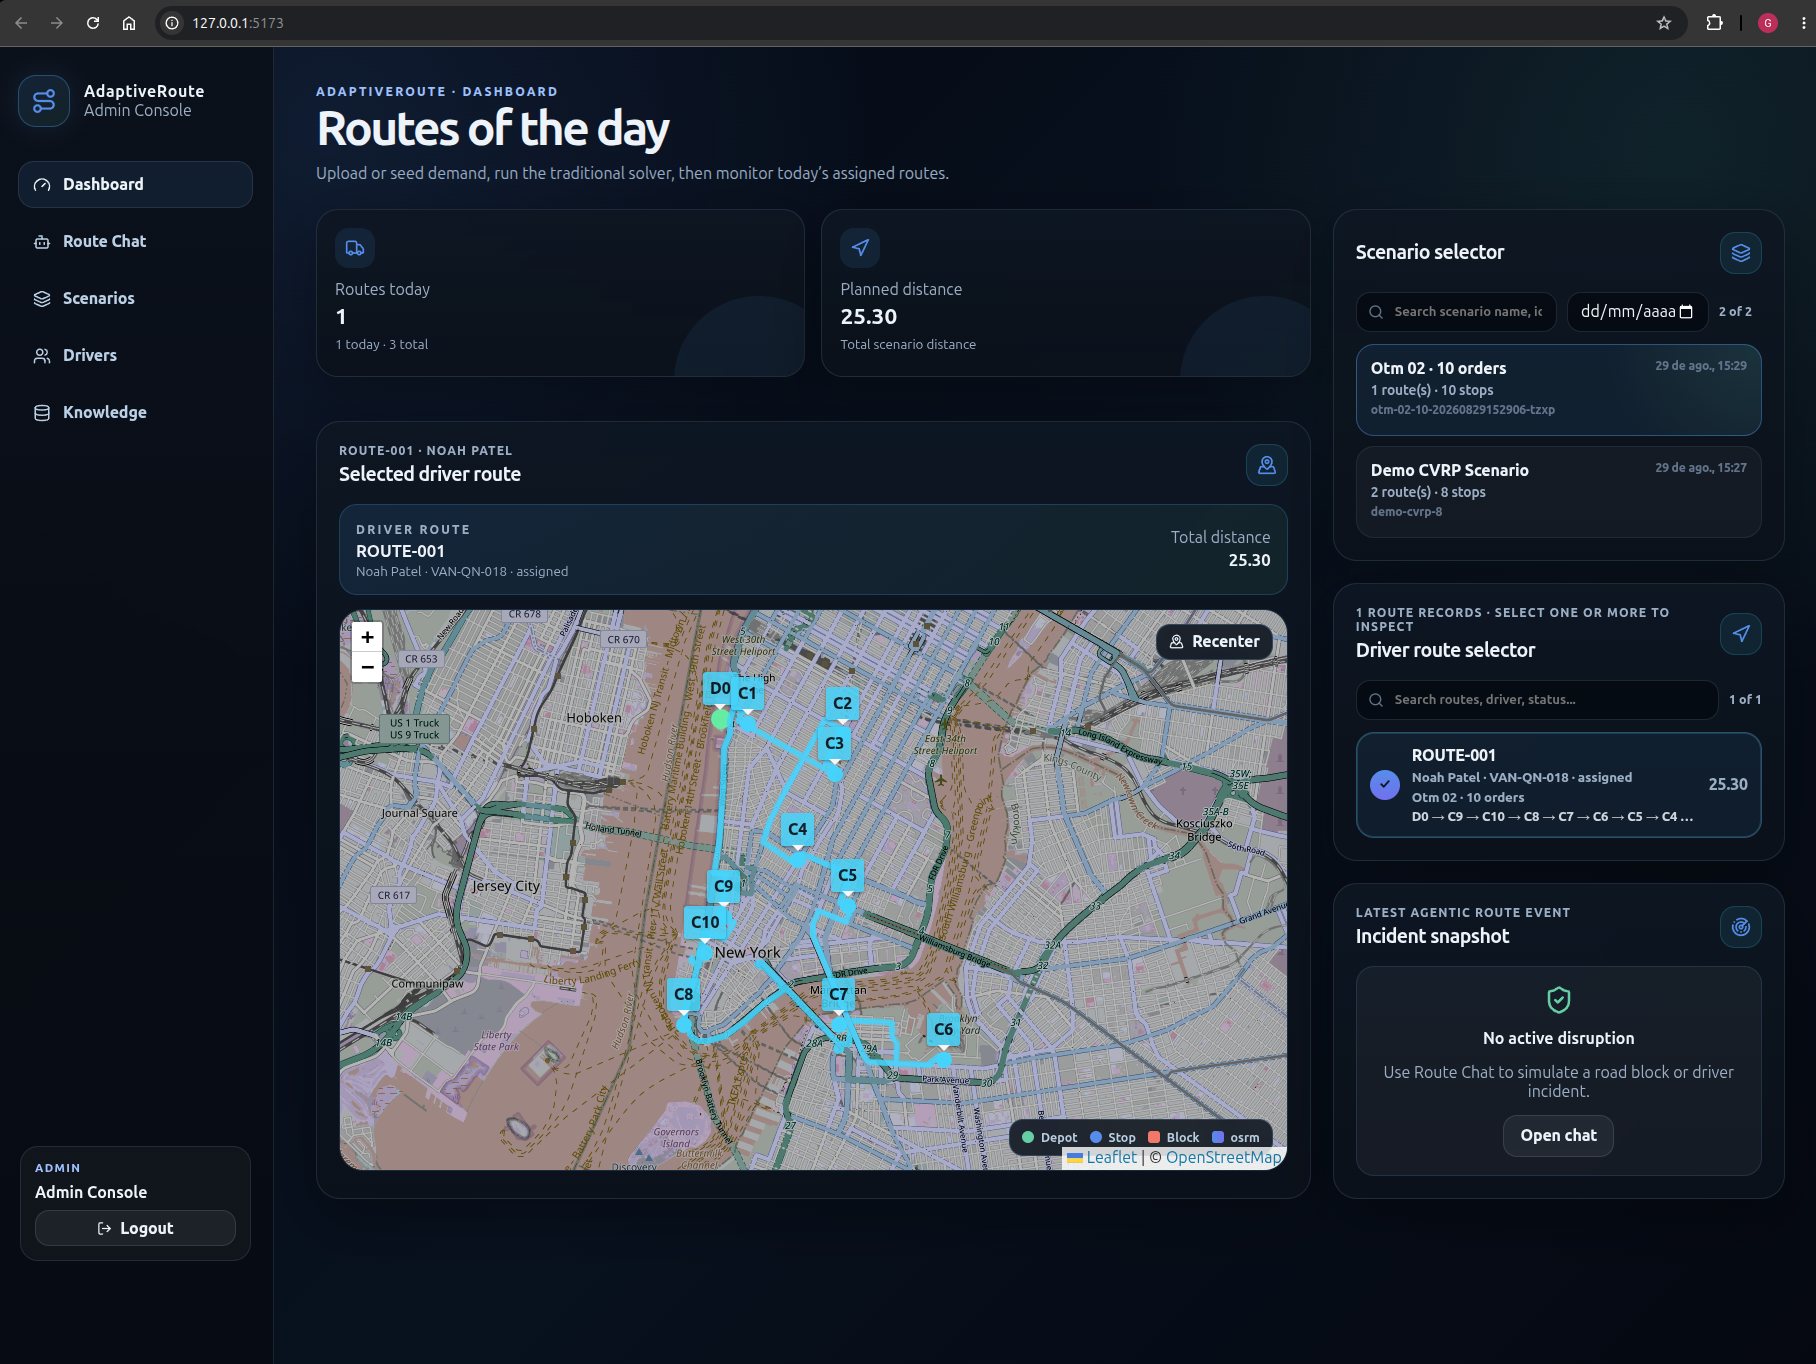
\includegraphics[width=\linewidth,height=0.84\textheight,keepaspectratio]{img/admin-dashboard.png}
    \end{column}
    \begin{column}{0.255\linewidth}
      \callout{Real road routing}{Geometry snapped to the street network by OSRM, not straight lines
      between stops.}\\[1.1em]
      \callout{Fleet and scenarios}{Orders ingested, scenarios persisted, routes assigned to named
      drivers.}\\[1.1em]
      \callout{Disruption watch}{The incident panel is where a driver's report surfaces on the
      operations side.}
    \end{column}
  \end{columns}

  \note{Worth pointing at the map legend: the ``osrm'' tag means these are real road distances and
  real geometry. Without OSRM the system still works --- it falls back to haversine and straight-line
  geometry --- which is fine for the maths but looks obviously synthetic on screen.}
\end{frame}

% ================================================================ 10 agent at work
\begin{frame}
  \frametitle{Everything so far, running}
  \framesubtitle{AdaptiveRoute \textperiodcentered\ The agent at work}

  \vspace{0.3em}
  \begin{columns}[c]
    \begin{column}{0.72\linewidth}
      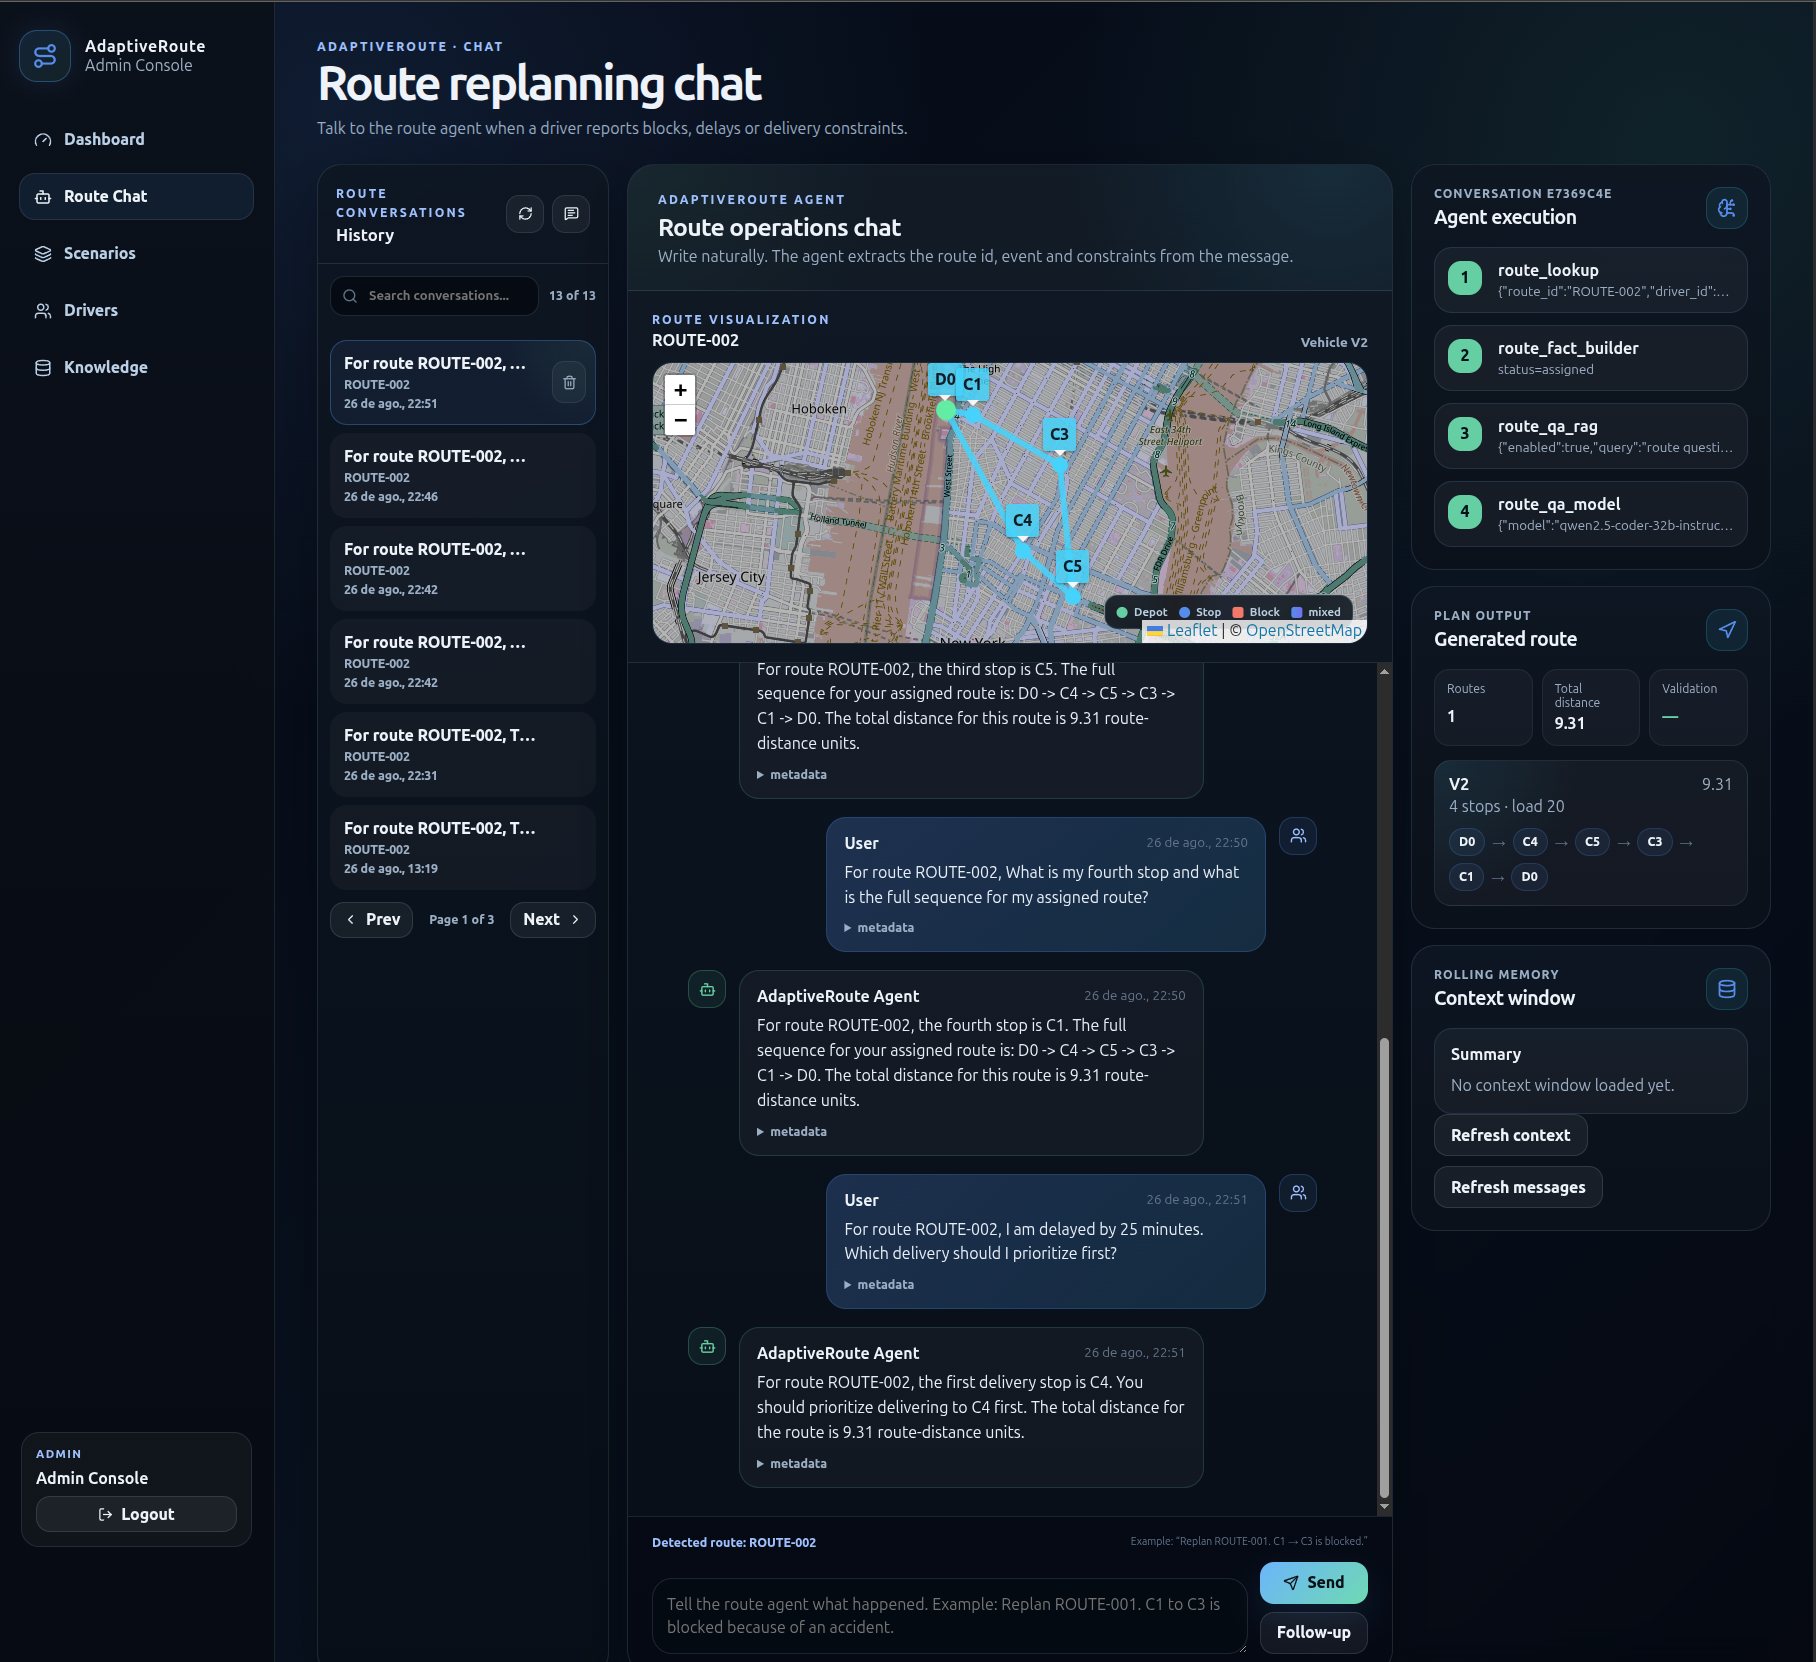
\includegraphics[width=\linewidth,height=0.84\textheight,keepaspectratio]{img/route-chat.png}
    \end{column}
    \begin{column}{0.255\linewidth}
      \callout{Agent execution}{The trace from the validation slide, step by step: lookup, fact
      builder, retrieval, model.}\\[1.1em]
      \callout{Validated plan}{Route, total distance and validation state --- the contract,
      enforced.}\\[1.1em]
      \callout{Rolling memory}{Context window carrying facts and constraints across the
      conversation.}
    \end{column}
  \end{columns}

  \note{This is the slide to linger on. The right-hand column is the architecture made visible: the
  execution trace is the LangGraph workflow, the plan output is the validation contract, and the
  context window is what lets a driver say ``and what about the next stop?'' without repeating
  themselves. The conversation itself is ordinary language --- no commands, no syntax.}
\end{frame}

% ================================================================ 11 training
\begin{frame}
  \frametitle{Supervised fine-tuning where\\ the optimiser is the teacher}
  \framesubtitle{AdaptiveRoute \textperiodcentered\ Building the routing policy}

  \vspace{0.6em}
  \begin{columns}[T]
    \begin{column}{0.478\linewidth}
      \begin{panel}{\linewidth}
        \plabel{How training data is made}\\[0.6em]
        \small
        \begin{enumerate}\setlength\itemsep{0.25em}
          \item Generate a synthetic CVRP instance
          \item Solve it to optimality with HiGHS
          \item Inject an operational event
          \item \cy{Re-solve} the disrupted scenario
          \item Validate, then serialise the pair
        \end{enumerate}
        \vspace{0.6em}
        \faint{The solver labels its own training set. The model learns to imitate optimal
        replanning, not to invent it.}
      \end{panel}
    \end{column}
    \begin{column}{0.478\linewidth}
      \begin{panel}{\linewidth}
        \plabel{Configuration}\\[0.7em]
        \color{arMuted}\footnotesize
        \begin{tabular}{@{}l@{\hspace{1.2em}}r@{}}
          Base model    & \color{arText}\bfseries Qwen2.5-7B-Instruct \\
          Method        & \color{arText}\bfseries LoRA / QLoRA \\
          Rank $r$      & \color{arText}\bfseries 16 \\
          Alpha         & \color{arText}\bfseries 32 \\
          Dropout       & \color{arText}\bfseries 0.05 \\
          Quantisation  & \color{arText}\bfseries 4-bit NF4 \\
          Compute dtype & \color{arText}\bfseries bfloat16 \\
          Epochs        & \color{arText}\bfseries 1 \\
          Hardware      & \color{arText}\bfseries RTX 3090 \textperiodcentered\ 24\,GB \\
        \end{tabular}\\[0.8em]
        \faint{Only the routing policy is fine-tuned. The orchestrator stays off the shelf.}
      \end{panel}
    \end{column}
  \end{columns}
\end{frame}

% ================================================================ 9 results
\begin{frame}
  \frametitle{Four variants, one fixed benchmark}
  \framesubtitle{AdaptiveRoute \textperiodcentered\ Model iteration}

  \vspace{0.1em}
  \muted{1{,}000 held-out scenarios, identical across every run.}

  \vspace{1.0em}
  \centering
  \small
  \begin{tabular}{@{}llrrrr@{}}
    \toprule
    \rowcolor{arBg}
    \color{arCyan}\scriptsize\bfseries &
    \color{arCyan}\scriptsize\bfseries TRAINING DATA &
    \color{arCyan}\scriptsize\bfseries FEASIBLE &
    \color{arCyan}\scriptsize\bfseries CAPACITY &
    \color{arCyan}\scriptsize\bfseries BLOCKED ARC &
    \color{arCyan}\scriptsize\bfseries EXACT \\
    \midrule
    \color{arText}v3 & \muted{30K compact curriculum}     & \muted{91.7\%} & \muted{72} & \muted{11} & \muted{4.6\%} \\
    \color{arText}v4 & \muted{+ 70K hard continuation}    & \muted{92.9\%} & \muted{61} & \muted{10} & \muted{\textbf{5.8\%}} \\
    \rowcolor{arPanel2}
    \color{arCyan2}\bfseries v5 & \color{arText}\bfseries + 20K error-driven &
      \color{arText}\bfseries 94.4\% & \color{arText}\bfseries 46 &
      \color{arText}\bfseries 9 & \color{arText}\bfseries 5.6\% \\
    \color{arText}v6 & \muted{+ 10K further error-driven} & \muted{94.0\%} & \muted{50} & \muted{10} & \muted{5.4\%} \\
    \bottomrule
  \end{tabular}

  \vspace{1.2em}
  \begin{minipage}{0.90\linewidth}
    \raggedright
    \cy{v5 selected.} Highest feasibility, fewest violations of both kinds, 100\% valid JSON
    everywhere. \muted{v6 confirmed the curve had flattened.}
  \end{minipage}

  \note{Exact match is deliberately not the decision metric --- a CVRP instance usually admits
  several equally optimal plans, so matching the reference sequence measures conformity, not quality.
  That is why v4 leads on exact match (5.8\%) but v5 is the right pick: it wins on every metric that
  describes whether the plan can actually be driven.}
\end{frame}

% ================================================================ 10 capacity
\begin{frame}
  \frametitle{Where the model stops working}
  \framesubtitle{AdaptiveRoute \textperiodcentered\ Capacity boundary}

  \vspace{0.1em}
  \muted{Measured, not estimated.}

  \vspace{0.9em}
  \begin{columns}[T]
    \begin{column}{0.46\linewidth}
      \centering\small
      \begin{tabular}{@{}rrl@{}}
        \toprule
        \color{arCyan}\scriptsize\bfseries CUSTOMERS &
        \color{arCyan}\scriptsize\bfseries VALID &
        \color{arCyan}\scriptsize\bfseries FAILURE MODE \\
        \midrule
        \color{arText}8  & \gn{100\%} & \muted{---} \\
        \color{arText}9  & \gn{100\%} & \muted{---} \\
        \color{arText}10 & \am{60\%}  & \muted{customer omitted} \\
        \color{arText}12 & \am{33\%}  & \muted{customer omitted} \\
        \color{arText}14 & {\color{arDanger}\bfseries 0\%} & \muted{customer omitted} \\
        \bottomrule
      \end{tabular}
      \vspace{0.7em}\\
      \faint{Small samples: 3--5 scenarios per size.}
    \end{column}
    \begin{column}{0.49\linewidth}
      \begin{panelglow}{\linewidth}
        \plabel{The boundary}\\[0.4em]
        {\color{arText}\Large\bfseries 8--9 customers}\\[0.5em]
        \muted{\small Above it the model omits customers --- it does not route them badly.}
      \end{panelglow}
      \vspace{0.8em}

      {\small A \cy{cardinality limit}, not a routing-quality problem. The fix is training data
      at 10--24 customers.}\\[0.6em]
      \faint{Beyond the boundary the plan is still correct --- the cascade falls through to the
      solver.}
    \end{column}
  \end{columns}

  \note{The omitted customers are the ones whose identifiers sit at the edge of the training
  distribution --- C10 and above, which the model rarely saw. That is why this reads as a
  generalisation failure rather than an optimisation failure, and why a better prompt does not fix
  it. Note the samples are small: 3--5 scenarios per size.}
\end{frame}

% ================================================================ 11 engineering
\begin{frame}
  \frametitle{What was built to make\\ the result trustworthy}
  \framesubtitle{AdaptiveRoute \textperiodcentered\ Engineering}

  \vspace{0.9em}
  \centering
  \stat{73}{Python modules,\\ $\sim$11{,}800 lines}\hfill
  \stat{24}{test files, runnable\\ without GPU or database}\hfill
  \stat{11}{architecture and\\ evaluation documents}

  \vspace{1.4em}
  \raggedright\small
  \begin{columns}[T]
    \begin{column}{0.47\linewidth}
      \begin{itemize}\setlength\itemsep{0.32em}
        \item[\color{arCyan}$\bullet$] Immutable domain model throughout
        \item[\color{arCyan}$\bullet$] Service / repository separation
        \item[\color{arCyan}$\bullet$] Protocol interfaces at every seam
      \end{itemize}
    \end{column}
    \begin{column}{0.47\linewidth}
      \begin{itemize}\setlength\itemsep{0.32em}
        \item[\color{arCyan}$\bullet$] CI split: fast API and forked solver tests
        \item[\color{arCyan}$\bullet$] bcrypt credentials, signed JWT, scoped CORS
        \item[\color{arCyan}$\bullet$] Structured logs with request ids
      \end{itemize}
    \end{column}
  \end{columns}
\end{frame}

% ================================================================ 12 limits
\begin{frame}
  \frametitle{What we would fix before\\ anyone depends on this}
  \framesubtitle{AdaptiveRoute \textperiodcentered\ Known limits}

  \vspace{0.7em}
  \begin{columns}[T]
    \begin{column}{0.478\linewidth}
      \begin{panel}{\linewidth}
        \plabel{Scale}\\[0.5em]
        \muted{\small MTZ relaxation is weak. Solver calls still run inside the request.}
      \end{panel}
      \vspace{0.8em}
      \begin{panel}{\linewidth}
        \plabel{Data}\\[0.5em]
        \muted{\small Fully synthetic. No real traffic, telemetry or road network.}
      \end{panel}
    \end{column}
    \begin{column}{0.478\linewidth}
      \begin{panelglow}{\linewidth}
        \plabelam{The unguarded edge}\\[0.5em]
        \ptitle{Validation covers the plan,\\ not the question}\\[0.6em]
        \muted{\small It proves the plan is right \emph{for the mutated scenario} --- not that the
        mutation matches what the driver said.}\\[0.7em]
        \am{This is the next thing to close.}
      \end{panelglow}
    \end{column}
  \end{columns}

  \note{On scale: OR-Tools or a branch-and-cut formulation for larger fleets, and a worker queue so
  optimisation leaves the request path. On the unguarded edge: event extraction is the one stage the
  trust boundary does not cover --- a misread message produces a perfectly valid answer to the wrong
  question, and no amount of plan validation can catch that.}
\end{frame}

% ================================================================ 13 next
\begin{frame}
  \frametitle{In priority order}
  \framesubtitle{AdaptiveRoute \textperiodcentered\ Next steps}

  \vspace{1.6em}
  \Large
  \begin{enumerate}\setlength\itemsep{0.85em}
    \item[\color{arCyan}\bfseries 1.] \cy{Harden event extraction}
    \item[\color{arCyan}\bfseries 2.] \cy{Push the cardinality boundary}
    \item[\color{arCyan}\bfseries 3.] \cy{Move optimisation off the request path}
    \item[\color{arCyan}\bfseries 4.] \cy{Instrument the cascade in production}
    \item[\color{arCyan}\bfseries 5.] \cy{Validate against real operations}
  \end{enumerate}

  \note{1 --- confidence thresholds and explicit confirmation before mutating a scenario.
  2 --- curriculum training at 10--24 customers; evaluate by scenario size, not a random split.
  3 --- worker queue, persisted solver artifacts, tuned time limits per scenario class.
  4 --- track fallback rate and violation modes; they are the live measure of model quality.
  5 --- replace synthetic scenarios with historical routes and observed disruptions.}
\end{frame}

% ================================================================ 14 close
\begin{frame}
  \frametitle{The system stays correct\\ when the model is wrong}
  \framesubtitle{AdaptiveRoute \textperiodcentered\ What the proof of concept established}

  \vspace{1.3em}
  \large
  \begin{itemize}\setlength\itemsep{0.75em}
    \item[\color{arCyan}$\bullet$] The routing policy returns \gn{94.4\% feasible replans} at the
          size it was trained for
    \item[\color{arCyan}$\bullet$] The remaining \cy{5.6\% is harmless} --- validation, repair, fallback
    \item[\color{arCyan}$\bullet$] A measured boundary of \cy{8--9 customers}, not an assumed one
    \item[\color{arCyan}$\bullet$] Natural language to validated route, \cy{end to end}
  \end{itemize}

  \vspace{1.8em}
  \normalsize
  \centering
  \faint{Built in five days. The interesting result is not the model --- it is everything built around it.}

  \note{The claim is deliberately narrow: feasible at the size it was trained for. The architectural
  claim is the broader one --- because the system never relies on the model being right, the failure
  rate stops being a risk and becomes a latency cost. And this is a working pipeline rather than a
  demonstration of components: one message in, one validated route out.}
\end{frame}

\end{document}
